Ada beberapa model algoritma yang sudah disediakan openCV untuk melakukan pengenalan wajah, diantaranya adalah
Eigenface, Fisherfaces, dan \emph{Local binary Pattern Histogram}(LBPH). Berikut penjelasan untuk perbedaan dari ketiga model algoritma yang disediakan olen openCV.
\section{Eigenface}

Eigenface adalah salah satu algoritma pengenalan wajah yang berdasarkan pada Principle Component Analysis (PCA) yang dikembangkan di MIT.
Algoritma EigenFace secara keseluruhan cukup sederhana, Training Image direpresentasikan dalam sebuah vektor flat (gabungan vektor) dan digabung
bersama-sama menjadi sebuah matriks tunggal. Eigen Vector kemudian diekstraksi dan disimpan dalam file temporary atau database. Training image
kemudian diproyeksikan dalam feature space yang di namai face space yang ditentukan oleh eigen vektor(Mukti, 2008).\footnote{Alam, R.G guntur, dkk.
\emph{MPLEMENTASI ALGORITMA EIGENFACE UNTUK FACE RECOGNITION PADA OBJECK FOTO ID CARD}.Telematik : Vol 7, No 2, April 2015.}
%http://repository.unib.ac.id/18865/1/4.%20IMPLEMENTASI%20ALGORITMA%20EIGENFACE%20UNTUK%20FACE.pdf

Principal Component Analysis (PCA) atau disebut juga transformasi KarhunenLoeve adalah tekhnik yang digunakan untuk menyederhanakan suatu data, dengan cara mentransormasi linear sehingga terbentuk
system koordinat baru dengan variansi maksimum. PCA dapat digunakan untuk mereduksi dimensi suatu data tanpa mengurangi karakteristik data tersebut secara signifikan (Cahyadi, 2007: 93)
\footnote{Firliana, Lina, dkk.\emph{Implementasi Principal Component Analysis (PCA) Untuk Pengenalan Wajah Manusia}. Universitas Nusantara}\\

Berikut proses langkah-langkah pengenalan wajah menggunakan model algoritma Eigenface.
\begin{enumerate}[1. ]
    \item Penyusunan flat vektor matriks
    \item Mengambil nilai tengah dari kumpulan matriks
    \item Menghitung selisih antara nilai matriks \emph{training image} dengan nilai tengah
    \item Menghitung nilai matriks kovarian
    \item Menghitung nilai \emph{eigenvalue} dan \emph{eigenvector}
    \item Menghitung nilai \emph{eigenface}
    \item Proses indentifikasi wajah 
\end{enumerate}

\section{Local Binary Pattern Histogram(LBPH)}
Local Binary Patter(LBP) adalah salah satu dari metode yang  terkenal dalam mengenali sebuah objek. Dalam hal ini, cara yang digunakan adalah membedakan objek dengan background. 
Local Binary Patter Histogram(LBPH) adalah sebuah kombinasi algoritma antara LBP dengan Histogram of Oriented Gradients(HOG)

Karakteristik utama dari pengenalan wajah menggunakan metode ini adalah komposisi \emph{micro texture-pattern} yaitu suatu operator nonparametrik yang menggambarkan tata ruang lokal citra. 
LBPH didefinisikan sebagai perbandingan nilai biner piksel pada pusat citra dengan 8 nilai piksel disekelilingnya. Misal pada sebuah citra berukuran 3x3, nilai biner pada pusat citra dibandingkan dengan nilai sekelilingnya. 
Dengan cara mengurangkan nilai piksel pada pusat citra dengan nilai piksel disekelilingnya, jika hasilnya lebih atau sama dengan 0 maka diberi nilai 1 dan jika hasilnya kurang dari 0 maka diberi nilai 0. 
Setelah itu, disusun 8 nilai biner searah jarum jam atau sebaliknya dan diubah 8 bit biner ke dalam nilai desimal untuk menggantikan nilai piksel pada pusat citra.
\footnote{Al-aidid, Sayeed, dan S.Pamungkas, Daniel. Sistem Pengenalan Wajah dengan Algoritma Haar 
Cascade dan Local Binary Pattern Histogram. Politeknik Negeri Batam}

Berikut merupakan langkah-langkah proses kerja LBPH, dimulai dari proses LBP hinnga selanjutnya dilakukan ekstraksi histogram dengan metode \emph{Histogram of Oriented Gradients} (HOG).\footnote{Kosasis, Rifki, dan Daomara, Christian. Pengenalan Wajah dengan Menggunakan Metode Local Binary 
Patterns Histograms (LBPH). Universitas Gunadarma}

Proses algoritma LBP terdiri dari 6 langkah, yaitu:
\begin{enumerate}
    \item Ubah citra wajah menjadi citra \emph{grayscale} dengan range intensitas pikselel adalah 0-255
    \item Membagi citra wajah menjadi bagian-bagian kecil yang disebut dengan sel, di mana tiap sel berukuran 3x3 piksel. 
        Karena setiap sel berukuran 3x3 maka banyaknya tetangga (P) adalah 8 dan radius (R) dari piksel tengah adalah 1
    \item Tentukan nilai pusat dari tiap sel, yaitu piksel tengah untuk digunakan sebagai nilai ambang. Nilai tersebut digunakan untuk menentukan nilai-nilai baru dari ke-8 piksel disekitarnya(piksel tetangga)
    \item Untuk setiap piksel tetangga dari piksel tengah , akan ditetapkan nilai biner baru dengan aturan 1 untuk nilai yang sama atau lebih tinggidari ambang, dan 0 untuk nilai lebih rendah dari nilai ambang
    \item Nilai piksel pada citra wajah selain piksel tengah hanya akan berisi nilai-nilai biner. Nilai tersebut digabungkan dari setiap posisi mennjadi barisan biner baru yang berukuran 8 bit
    \item Kemudian, nilai biner ini akan dikonversikan ke nilai desimal dengan range 0-255, sehingga menghasilkan citra baru  yang mewakili karakteristik (fitur) dari citra asli dengan lebih baik.
\end{enumerate}

Setelah proses LBP dilakukan, selanjutnya dilakukan ekstraksi histogram dengan menggunakan metode \emph{Histogram of Oriented Gradients} (HOG). Pada metode HOG terdapat 4 langkah yaitu:
\begin{enumerate}
    \item Citra hasil LBP dibagi menjadi daerah-daerah kecil yang disebut dengan grid. 
    \item Buat histogram dari daerah tersebut
    \item Karena citra hasil LBP merupakan citra grayscale maka setiap histogram dari setiap grid hanya akan berisi 256 posisi (0-255) yang mewakili setiap intensitas piksel. 
    \item Histogram dari tiap daerah (grid) digabung menjadi satu histogram besar. Jika tiap grid berukuran 8x8, maka total memiliki 8x8x256 = 16,384 posisi dalam histogram akhir. 
    Histogram terakhir merupakan fitur yang mewakili citra asli dan diasumsikan sebagai sebuah vektor
\end{enumerate}
\begin{figure}[h!]
    \centering
    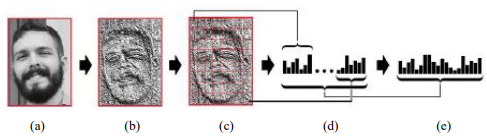
\includegraphics[width=0.7\linewidth]{images/lbph.PNG}
    \caption{Contoh Hasil LBPH}
\end{figure}

\newpage
\section{Fisherfaces}
Algoritma Fisherface ini merupakan gabungan dari metode Principal Component Analys (PCA) dengan Fisher’s Linear Discriminant (FLD). FLD merupakan salah satu contoh metode class specific, 
karena prinsip dasar metode ini berusaha untuk membentuk jarak (scatter) antar kelas dan intra kelas sehingga dapat menghasilkan klasifikasi yang lebih baik, dan mereduksi dimensi yang didapat dari perhitungan PCA. 
Semakin besar rasio antar kelas, vector ciri yang dihasilkan semakin tidak sensitive terhadap perubahan ekspresi maupun perubahan pencahayaan, sehingga dapat menghasilkan klasifikasi yang lebih baik. 
\footnote{Amalia, Nurul. Perbandingan Algoritma Fisherface dan Algoritma Local Binary Pattern Untuk Pengenalan Wajah. Universitas Budi Darma, Medan}
\begin{figure}[h!]
    \centering
    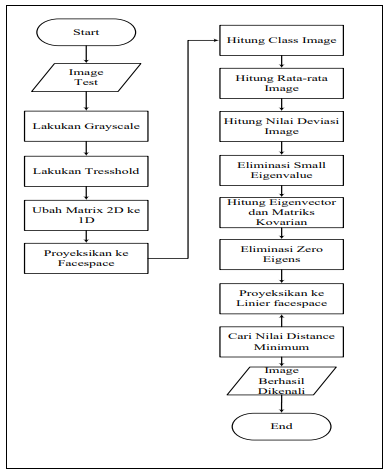
\includegraphics[width=0.7\linewidth]{images/algoritma_fisherface.PNG}
    \caption{Proses algoritma fisherface}
\end{figure}